% !TEX root = ../Ausarbeitung.tex
\section{Introduction}
In scope of the \textit{Praktikum} within the Human Brain Project, we work with the Neurorobotics Platform (NRP) which provides a simulation environment for robotics.
More specifically, our experiment setup consists of a table, on which a robot arm is placed.
The robot arm has a six joints and a hand with five fingers.
In front of the robot arm, a cylinder is placed on the table.
The goal of the Praktikum is to move the cylinder as far as possible with the robot arm.
This can be performed by just hitting the cylinder away or by grabbing the cylinder and throw it as far as possible.
The performance is measured by the distance of the cylinder.
In the following, several strategies to fulfill this task are presented.
These consist in a hard-coded approaches and in more sophisticated approaches using learning algorithms.
The setup is depicted in \autoref{fig:hbbprak_2018}.

\begin{figure}[h]
\centering
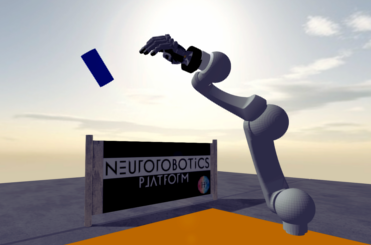
\includegraphics[width=.95\columnwidth]{figures/hbpprak_2018.png}
\caption{The goal is to throw the cylinder as far as possible.}
\label{fig:hbbprak_2018}
\end{figure}